\documentclass[a4paper,11pt]{report}
\usepackage[showexo=true,showcorr=false]{../packages/coursclasse}
%Commenter ou enlever le commentaire sur la ligne suivante pour montrer le niveau
\toggletrue{montrerNiveaux}
%permet de gérer l'espacement entre les items des env enumerate et enumitem
\usepackage{enumitem}
\setlist[enumerate]{align=left,leftmargin=1cm,itemsep=10pt,parsep=0pt,topsep=0pt,rightmargin=0.5cm}
\setlist[itemize]{align=left,labelsep=1em,leftmargin=*,itemsep=0pt,parsep=0pt,topsep=0pt,rightmargin=0cm}
%permet de gerer l'espacement entre les colonnes de multicols
\setlength\columnsep{20pt}

\begin{document}

%%%%%%%%%%%%%%%%% À MODIFIER POUR CHAQUE SERIE %%%%%%%%%%%%%%%%%%%%%%%%%%%%%
\newcommand{\chapterName}{Nombres et opérations}
\newcommand{\serieName}{Les critères de divisibilité}


%%%%%%%%%%%%%%%%%% PREMIERE PAGE NE PAS MODIFER %%%%%%%%%%%%%%%%%%%%%%%%
% le chapitre en cours, ne pas changer au cours d'une série
\chapter*{\chapterName}
\thispagestyle{empty}

%%%%% LISTE AIDE MEMOIRE %%%%%%
\begin{amL}{\serieName}{
\item Critères de divisibilité (page 13)
}
\end{amL}

%%%%%%%%%%%%%%% DEBUT DE LA SERIE NE PAS MODIFIER %%%%%%%%%%%%%%%%%%%%%%%%%%%%%
\section*{\serieName}
\setcounter{page}{1}
\thispagestyle{firstPage}



%%%%%%%%%%% LES EXERCICES %%%%%%%%%%%%%%%%%%%%%%%%%%%%%%%%%%%%

\begin{exol}{NO28}{17}{1}
\end{exol}

\begin{exof}{NO29}{11}{2}
\end{exof}

\begin{exol}{NO37}{19}{2}
\end{exol}

%----------------------------------------------------------------
\begin{exop}{
    Parmi les nombres suivants, entoure les multiples de $2$.
    \begin{tasks}(7)
\task[] $260$ 
\task[] $8565$ 
\task[] $840$ 
\task[] $9753$ 
\task[] $6254$ 
\task[] $2738$ 
\task[] $9607$
    \end{tasks}
}{1}\end{exop}

\begin{exop}{
    Parmi les nombres suivants, entoure les multiples de $3$. 
    \begin{tasks}(7)
\task[] $858$ 
\task[] $4256$ 
\task[] $639$ 
\task[] $7344$ 
\task[] $6257$ 
\task[] $4228$ 
\task[] $1243$
    \end{tasks}
}{1}\end{exop}




%----------------------------------------------------------------
\begin{exop}{
    Parmi les nombres suivants, entoure les multiples de $5$. 
    \begin{tasks}(7)
\task[] $3246$ 
\task[] $6240$ 
\task[] $6298$ 
\task[] $4285$ 
\task[] $573$ 
\task[] $8275$ 
\task[] $6350$
    \end{tasks}
}{1}\end{exop}



%-------L'élève découvre l'inclusion M3<M9-------------------------------------
\begin{exop}{
    En rouge, entoure les nombres divisibles par 3. 

    En vert, entoure les nombres divisibles par 9.

    \begin{tasks}(6)
\task[]    $18$ 
\task[] $60$ 
\task[] $178$ 
\task[] $216$ 
\task[] $32$ 
\task[] $81$ 
\task[] $192$
\task[] $1725$ 
\task[] $3960$ 
\task[] $371$ 
\task[] $687$ 
\task[] $0$
    \end{tasks}
}{1}\end{exop}





%--------------------------------------------------------------------
\begin{exop}{
    Parmi les nombres suivants, entoure les nombres qui sont à la fois multiples de $2$ et de $3$.

    Vérifie à l'aide de ta calculatrice qu'ils sont multiples de $6$. 

    \begin{tasks}(7)
\tasks[] $4258$ 
\task[] $369$ 
\task[] $6246$ 
\task[] $126$ 
\task[] $458$ 
\task[] $735$ 
\task[] $264$
    \end{tasks}
}{1}\end{exop}





%---------------------------------------------------------------
\begin{exop}{
    Parmi les nombres suivants, entoure les nombres qui sont à la fois multiples de $2$ et de $5$. 

    Vérifie qu'ils sont multiples de $10$.

    \begin{tasks}(7)
\task[] $625$ 
\task[] $3420$ 
\task[] $728$ 
\task[] $4250$ 
\task[] $747$ 
\task[] $820$ 
\task[] $5256$
    \end{tasks}
}{1}\end{exop}


%---------------------------------------------------------------
\begin{exop}{
    Parmi les nombres suivants, entoure les nombres qui sont à la fois multiples de $3$ et de $5$. 

    Vérifie à l'aide de ta calculatrice qu'ils sont multiples de $15$.

    \begin{tasks}(7)
\task[]   $4260$ 
\task[] $525$ 
\task[] $636$ 
\task[] $175$ 
\task[] $840$ 
\task[] $6235$ 
\task[] $8310$
    \end{tasks}
}{1}\end{exop}






%--------------------------------------------------------------
\begin{exo}{
    Quel nombre divisible par 3 est le plus près des nombres suivants~?
    \begin{tasks}(4)
	    \task[] $397$
	    \task[] $1235$
	    \task[] $8567$
	    \task[] $68234$
\end{tasks}
}{2}\end{exo}


%------------------------------------------------------
\begin{exo}{
    Trouve un nombre de 3 chiffres compris entre 152 est 167 qui soit divisible par 5 et par 3.
}{2}\end{exo}





%--------------------------------------------------------------
\begin{exo}{
    Les affirmations suivantes sont-elles vraies ou fausses~? Justifie chacune de tes réponses.

    \begin{tasks}
    \task Tous les nombres qui se terminent par 3 sont divisibles par 3.
    \task Les nombres divisibles par 3 sont tous impairs.
    \task Tous les nombres pairs sont divisibles par 2.
    \task Un nombre qui se termine par 4 est toujours divisible par 2.
    \task Un nombre divisible par 2 se termine forcément par 4.
    \task Tous les nombres divisibles par 5 sont impairs.
    \end{tasks}

}{3}\end{exo}


%---------------------------------------------------------------
\begin{exop}{
    En rouge, entoure les nombres divisibles par 10. 

    En vert, entoure les nombres divisibles par 25.

    En bleu, entoure les nombres divisibles par 100.

    \begin{tasks}(7)
\task[] $180$ 
\task[] $600$ 
\task[] $178$ 
\task[] $225$ 
\task[] $32$ 
\task[] $50$ 
\task[] $190$
\task[] $1725$ 
\task[] $3960$ 
\task[] $3700$ 
\task[] $687$ 
\task[] $0$ 
\task[] $175$
\task[] $1010$
    \end{tasks}
}{1}\end{exop}



%---------------------------------------------------------------
\begin{exo}{ 
    \begin{tasks}
    \task Parmi les entiers ci-dessous, lesquels sont des multiples de 4~?
        \begin{center}
            $4266$ \hspace*{1.3cm} $7650$ \hspace*{1.3cm} $33684$ \hspace*{1.3cm} $636200$ \hspace*{1.3cm} $75240$
        \end{center}
            
	\vspace{-0.2cm}      

\task Remplace chaque carré par un chiffre, de manière à obtenir un multiple de 4. Indique toutes les possibilités. 
\end{tasks}
\begin{center}
{\large $\square~8~2~5~\square$}
\end{center}
}{3}\end{exo}

	\begin{qmoodle}{Critères de divisibilité
}{2}{
	\begin{center}	
		Q1


\includegraphics[scale=1]{media/qr/necd1 }

\tiny{{https://edu.ge.ch/qr/necd1}}
\end{center}
	\begin{center}	
		Q2


\includegraphics[scale=1]{media/qr/necd2 }

\tiny{{https://edu.ge.ch/qr/necd2}}
\end{center}
}
\end{qmoodle}



%--------------------------------------------------------------
\begin{exo}{
    Dans un nombre de 8 chiffres {\large \[1~\square~9~\square~9~\square~5~\square \] }On doit remplacer les cases par des chiffres pour que le nombre obtenu soit divisible par 2; 5 et 9.

    Combien de nombres différents peut-on fabriquer à ces conditions~?
    \begin{tasks}(5)
    	\task 111 
     	\task 115 
	\task 104 
	\task 102 
	\task 81
\end{tasks}
}{3}\end{exo}


%--------------------------------------------------------------
\begin{resolu}{Critère de divisibilité par 7}{
    Voici un critère de divisibilité par 7 donné à l'aide d'un organigramme. On choisit un entier $N$ supérieur à 70 (on reconnaît immédiatement les multiples de 7 jusqu'à 70).

    \begin{center}




\begin{tikzpicture}[scale=1]
% définition des styles
%\tikzstyle{estun}=[->,>=latex,very thick,dotted]
% les nœuds
\node[rectangle, draw] (A) at (0,0) {Entrer l'entier $N$};
\node[rectangle, draw] (B) at (0,-1.5) {Supprimer le dernier chiffre};
\node[rectangle, draw,,text width=6.5cm] (C) at (0,-3.5) {Soustraire le double du chiffre qu'on vient de supprimer};
\node[ellipse, draw, text width=5.5cm] (D) at (0,-6) {Le résultat obtenu est-il supérieur à 70 ?};
\node[ellipse, draw, text width=5.5cm] (E) at (0,-9) {Le résultat obtenu est-il 0 ou un multiple de 7 ?};
\node[rectangle, draw, fill=red!50, text width=3cm] (N) at (8,-9) {$N$ n'est pas un multiple de 7};
\node[rectangle, draw, fill=green!50] (O) at (0,-11.5) {$N$ est un multiple de 7};
% les flèches
\draw[>=latex, ->, very thick] (A)--(B);
\draw[>=latex, ->, very thick] (B)--(C);
\draw[>=latex, ->, very thick] (C)--(D);
\draw[>=latex, ->, very thick] (D)--(-6,-6)node[midway,above]{oui} ;
\draw[>=latex, ->, very thick] (-6,-6)|-(B) ;
\draw[>=latex, ->, very thick] (D)--(E)node[midway,right]{non};
\draw[>=latex, ->, very thick] (E)--(O)node[midway,right]{oui};
\draw[>=latex, ->, very thick] (E)--(N)node[midway,above]{non};

\end{tikzpicture}

\end{center}

\begin{tasks}
    \task 25802 est-il divisible par 7~?
    {\color{blue}
	    \begin{align*}
		    2580-4&=2576 &&\text{ (car }2\cdot2=4) \\
		    257-12&=245 &&\text{ (car }2\cdot6=12) \\
		    24-10&=14 &&\text{ (car } 2\cdot5=10)
\end{align*}   
14 est un multiple de 7. Ainsi, 25802 est un multiple de 7.}
    \task 67693 est-il divisible par 7~?
    {\color{blue}
	    \begin{align*}
		    6769-6&=6763 &&\text{(car }2\cdot3=6) \\
		    676-6&=670 &&\text{(car }2\cdot3=6) \\
		    67-0&=67 &&\text{(car }2\cdot0=0)
\end{align*}
    67 n'est pas un multiple de 7. Ainsi, 67693 n'est pas un multiple de 7.}
\end{tasks}
}{3}\end{resolu}

\begin{exo}{
Parmi les entiers ci-dessous, lesquels sont des multiples de 7~? Aide-toi de l'exercice résolu ci-dessus. 
\begin{tasks}(3)
	\task[] $251$ \task[] $2576$ \task[] $4575$ \task[] $4888$ \task[] $347102$ \task[] $46860$
\end{tasks}
}{3}\end{exo}



%--------------------------------------------------------------
\begin{resolu}{Critère de divisibilité par 11}{
    Un entier positif est divisible par 11 si la différence entre la somme des chiffres de rang impair et la somme des chiffres de rang pair est 0 ou un multiple de 11. Sinon, il n'est pas divisible par 11.

    \begin{tasks}
        \task 613470 est-il divisible par 11~? 
        
        {\color{blue}
        \begin{center} 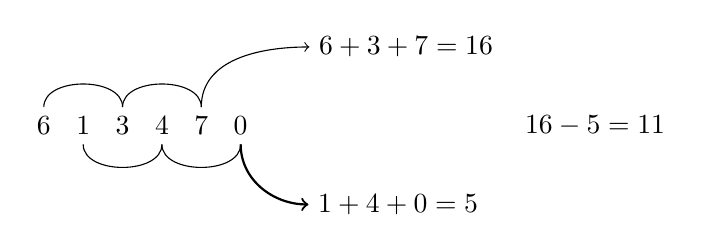
\begin{tikzpicture}
\node[] (A) at (0,0) {6};
\node[] (B) at (0.5,0) {1};
\node[] (C) at (1,0) {3};
\node[] (D) at (1.5,0) {4};
\node[] (E) at (2,0) {7};
\node[] (F) at (2.5,0) {0};

\node[] (I) at (4.6,1) {$6+3+7=16$} ;
\node[] (P) at (4.5,-1) {$1+4+0=5$} ;

\node[] (R) at (7,0) {$16-5=11$};

\draw[] (A)to[out=90,in=90](C);
\draw[] (C)to[out=90,in=90](E);
\draw[] (B)to[out=-90,in=-90](D);
\draw[] (D)to[out=-90,in=-90](F);
\draw[->] (E)to[out=90,in=180](I) ;
\draw[thick, ->] (F)to[out=-90,in=180](P);
\end{tikzpicture}
\end{center}
        \hspace*{.8cm} Oui, 613470 est divisible par 11.}
        
        \task 3285341 est-il divisible par 11~?
        {\color{blue}
        \begin{center} 
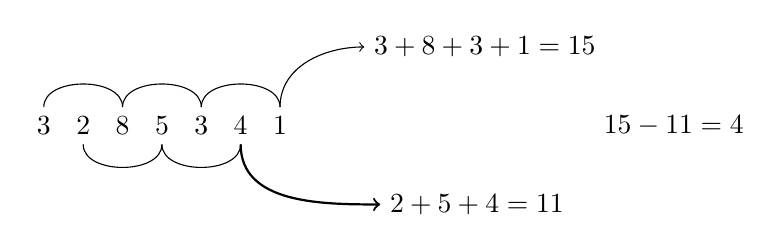
\begin{tikzpicture}

\node[] (A) at (0,0) {3};
\node[] (B) at (0.5,0) {2};
\node[] (C) at (1,0) {8};
\node[] (D) at (1.5,0) {5};
\node[] (E) at (2,0) {3};
\node[] (F) at (2.5,0) {4};
\node[] (G) at (3,0) {1};

\node[] (I) at (5.6,1) {$3+8+3+1=15$} ;
\node[] (P) at (5.5,-1) {$2+5+4=11$} ;

\node[] (R) at (8,0) {$15-11=4$};

\draw[] (A)to[out=90,in=90](C);
\draw[] (C)to[out=90,in=90](E);
\draw[] (E)to[out=90,in=90](G);
\draw[] (B)to[out=-90,in=-90](D);
\draw[] (D)to[out=-90,in=-90](F);
\draw[->] (G)to[out=90,in=180](I) ;
\draw[thick, ->] (F)to[out=-90,in=180](P);

\end{tikzpicture}
\end{center}
        \hspace*{.8cm}Non, 3285341 n'est pas divisible par 11.}
        
    \end{tasks}
}{3}\end{resolu}

%\includegraphics[width=0.8\textwidth]{images/critere11.png}
\begin{exo}{
\begin{tasks}
    \task Parmi les entiers ci-dessous, lesquels sont des multiples de 11~? Aide-toi de l'exercice résolu ci-dessus.
\end{tasks}
    \begin{tasks}(6)    
\task[] $1408$ 
\task[] $2812$ 
\task[] $40161$ 
\task[] $71968$ 
\task[] $394317$ 
\task[] $138477$
\end{tasks}
\begin{tasks}
	\task[b)] Remplace chaque carré par un chiffre, de manière à obtenir un nombre divisible par 11. Indique toutes les possibilités.
	    {\large
	    \begin{align*}
		    &\square~2~4~6~3~\square  && 3~6~\square~2~9\\
		    &\square~2~\square~3~8   &&5~\square~\square~3~6
\end{align*}}

\end{tasks}
}{3}\end{exo}

\end{document}

